%%
%% neuralfields.tex
%% 
%% Made by jjfigueredou
%% Login   <jjfigueredou@fctp-jjfu>
%% 
%% Started on  Sun Oct  5 12:26:22 2008 jjfigueredou
%% Last update Sun Oct  5 12:26:22 2008 jjfigueredou
%%
\documentclass[preprint]{sigplanconf}
\usepackage[latin1]{inputenc}
\usepackage[numbers]{natbib}
\usepackage[english]{babel}
\usepackage{graphicx}
\usepackage{algorithm}
\usepackage{algorithmic}
\usepackage{amsmath}

\begin{document}
\conferenceinfo{}{} \copyrightyear{} \copyrightdata{[to be supplied]}

\titlebanner{PREPRINT} % These are ignored unless
\preprintfooter{DRAFT} % 'preprint' option specified.

\title{Neural Fields Applied to the Stability Problem of a Simple
  Biped Walking Model}

\authorinfo{Juan J. Figueredo} {Departamento de Ingenier�a de Sistemas
  e Industrial, Universidad Nacional de Colombia.}
{jjfigueredou@unal.edu.co}

\date{\today}
\maketitle

\begin{abstract}
  The control problem in biped walking has shown to be quite complex,
  because of sits nonlinear dynamics. Several models have been
  developed to simplify gait behavior and several controllers have
  been developed around this problem. This article shows an approach
  to this problem by means of the inverted pendulum model, using a
  biological hypothesis of biped walking control in two
  subsystems. The first one is an equilibrium controller, and the
  second one is a path-following controller which achieves its
  behavior by perturbing the first one. Here we show how the first
  controller can be obtained using neural fields as control
  architecture without any inner parameterization, and compare its
  results with a recurrent neural network controller parameterized by
  an evolutionary algorithm. Finally, there are discussed some of the
  potential ways to extends the neural field architecture to face the
  complete problem of control of the simple walking model, or even
  harder problems, by using evolution.
\end{abstract}

\section{Introduction}
Artificial life aims to find those emergent phenomena that give
complex attributes to the existent living beings. In this work,
efforts are directed towards the study of emergence of motion control
capabilities and dynamical planning behaviors of biped walking
agents. Following the artificial life approach \cite{Nolfi}, those
capabilities are expected to evolve from a very simple or
non-functional initialization, in this case using a recurrent neural
network as control architecture. Nonetheless, adaptation can obtain a
great benefit from a representation or architecture which has a
structure well suited for the problem at hand. For a deeper insight
computational intelligence looks into nature.

Recurrent neural networks have some resemblance to our neural system:
they are a set computing units coupled in a topology or connection
scheme. They are known to be able to approximate any route on a
n-dimensional dynamical system with arbitrary accuracy
\cite{Funahashi93Approximation}. However, they do not have any
internal structure that is particularly suited to a control problem.

Neural fields have a closer similarity with our neural system: they
are tissue-level models of neural populations. They have a spacial
interpretation and generally requires a metric for the elements. Also,
its dynamic equation has a linear stabilizing terms
\cite{Ermentrout98Neural}. This properties and a standard connection
function (or kernel) were shown to be able to solve a kinematic
navigation problem \cite{Bergener99Complex}. Here we show how the
dynamic (kinetic) stability control problem for the simple biped
walking model can also be solved without additional parameterization
of the architecture.  Here, there are compared two control schemes
based on recurrent neural networks, in order to observe their
advantages and disadvantages as planning and control architectures and
their suitability to evolution. The first one, uses a simple model of
recurrent connections between neurons without additional
restrictions. The second one, neural fields, has a deeper biological
basis, applying more restrictions and extending the discrete model to
a continuous one, following the method of planning and control by
means of neural fields \cite{BBD99}.

Next, some preliminaries on computational intelligence are presented,
mainly in the areas of evolutionary computation, which is the main
focus of the article, and in the area of neural controllers. In the
remaining sections the control problem used as test bed is presented,
an application of traditional evolutionary computation methods is
shown, a co-evolution scheme is applied, other incremental evolution
methods are used to obtain greater complexity, and finally, a
discussion is made.


\section{Preliminaries on Computational Intelligence}
\subsection*{Evolutionary algorithms}
Evolutionary algorithms are a set of population-based heuristic search
and optimization techniques. They maintain a population, and apply a
set of operators or transformations over its members. Those operators
are typically inspired on biological evolution and usually include
selection, reproduction and mutation, among others. The operators are
dependent of the evaluation of a performance function called fitness
function. Generally, fitness function evaluation may include, from a
simple numerical evaluation, to a complex simulation, in order to get
the performance criterion which its optimization is pursued.

The pseudo-code of a general evolutionary algorithm is as follows:

\algsetup{indent=2em}
\begin{algorithm}[h!]
  \caption{$Evolutionary Algorithm$}\label{alg:factorial}
  \begin{algorithmic}[1]
    \STATE $P \leftarrow$ Generate initial population of size $N$
    \STATE Evaluate fitness for each individual in $P$ \REPEAT \STATE
    $P' \leftarrow$ Apply operators to $P$ \STATE Evaluate fitness for
    each individual in $P'$ \STATE $P \leftarrow$ Select $N$
    individuals in $P'$ according to a selection scheme
    \UNTIL{Termination condition is met}
  \end{algorithmic}
\end{algorithm}

The most predominant form of an evolutionary algorithm is embodied by
genetic algorithms. They most frequent genotypical representation is a
bit sequence, although other representations can be used. Usually they
are implemented with a generational replacement of population, but in
some situations it is useful to conserve a small set of the better
individuals across generations in a steady-steady replacement.

\subsection*{Recurrent neural networks and neural fields}
Artificial neural networks are a connectionist computing scheme
inspired by brain neural layout at cellular level. It is based on
simple computing structures called neurons which have several inputs
and a single output.

The particular topologies of interest here are recurrent neural
networks and neural fields.

For recurrent neural networks the model, as is presented in
\cite{Haykin99} is:

\begin{align}
  \begin{split}
    x_{rnn}(n+1)&=\Psi (W_ax_{rnn}(n)+W_bu_{rnn}(n)) \\
    y_{rnn}(n)&=Cx_{rnn}(n)
  \end{split}
\end{align}

Here, $x_{rnn}$ is the 1-by-q system state vector at $n$, $\Psi$ is a
diagonal function with domain and co-domain $R^q$ corresponding to
activation function, $u_{rnn}$ is the 1-by-m input vector at $n$, the
.q-by-q matrix $W_a$ represents the connection weights between
neurons, and the q-by-m+1 matrix represents the connection weights
between input nodes and neurons, including a bias term. Also,
$y_{rnn}$ is the neural output vector of the neural net, and $C$ is a
p-by-q matrix of linear combination from the neurons to the outputs.

Recurrent neural networks present a dynamic behavior because of its
memory, that is, each state depends of the previous state in such a
way that a difference equation arises. Here, there is not a notion of
locality and the interactions between neurons and inputs is given by
parameter matrices.


Neural fields, on the other hand, arise as a tissue level model of neural populations in
brain. It has been proposed by Wilson and Cowan \cite{Wilson72Excitatory} and detailed
by Amari \cite{Amari77Dynamics} in the particular case of lateral inhibition. In
this model, neural population in considered continuum in which exists
a dynamical evolution equation where the mean activation potential
evaluated in one place is affected by its neighborhood according to a
so-called mexican hat function (as noted by Coombes \cite{Coombes05Waves} better
called wizard hat function) in which close neighbors act as exciters
and distant ones act as inhibitors.

The base model, as presented by Amari \cite{Amari77Dynamics} for the multiple
layer case is:

\begin{equation}
  \label{eq:nf-base}
  \tau_i\frac{\delta u_i(x,t)}{\delta
    t}=-u_i+\sum_{j=1}^{m}{\int{w_{i,j}(x,x';t-t')f_j\left(
    u_j(x',t')\right) dx' dt'}+h_i+s_i(x,t)}
\end{equation}

Where $\tau$ is a temporal constant of synaptic decay rate, $u_i(x,t)$
is the average membrane potential of the neurons located at position
$x$ at time $t$ on layer $i$ (where $x$ can be 1-dimensional, 2-dimensional or even
of higher dimension). The average intensity of connection from neurons
on layer $j$ at $y$ to neurons on layer $i$ at $x$ is modeled with
$w_{i,j}(x,y)$, $f_j(\cdot)$ is the saturating output function which is
monotonically nondecreasing. The deviation of the average stimulation
potential at place $x$ at time $y$ of layer $i$ is represented by
$s_i(x,t)$, and $h_i=\bar{s_i}-r_i$ is the sum of the average
stimulation potential an the resting potential of layer $i$. 


The main difference between recurrent neural networks and neural
fields is that, in the first, the relation among the neurons is
arbitrary and discrete, but in the second is continuous and is meant
to be related to locality. Besides, the first right hand element
assures and stable homogeneous behavior in linear form.

\section{Evolution of Neural Field Controllers for Biped Walking}
\subsection*{Neural Field Controller Architecture}
The architecture used for the neural field controller uses a structure
similar to that of multilayer perceptrons, i.e. an input layer, a
hidden layer and an output layer. The hidden layer has the properties
so far presented in the neural field model. The input and output
layers are also modelled as a population of neurons but without inner
dynamics. Nonetheless, it is used a kernel for the connection from the
input layer to the hidden layer, as well for the connection from the
hidden layer to the output layer.  The input layer is used as a buffer
where sensory inputs are placed before they are processed by the
hidden layer. The output layer is used so that it can be applied some
form of post-processing to the output of the hidden layer without
changing the inner dynamics of the neural field.

\subsection*{Evolutionary Algorithm Structure and Parameters}
% \subsection*{Genotypic Representation and Evolution Operators}
For the evolution process it is used a simple evolutionary algorithm
as shown in the preliminaries, but with the addition of niching in the
for of Deterministic Crowding (see \cite{referencia-dc}), in order to
promote additional diversity and to prevent premature convergence.

The evolution parameters are the connection kernels between the input
layer and the hidden layer, and between the hidden layer and the
output layer. The recurrent connections of the hidden layer with
itself are left fixed, in the form of a wizard hat function.

The connection kernels are considered isotropic and homogeneous along
the field, so that they can be described as symmetric one-dimensional
arrays of values.

\subsection*{Fitness Functions}

The fitness functions were selected in such a way that the stability
controller only has the goal to reduce inclination, while the
positioning controller has to take into account both inclination and
position. The fitness functions were tuned experimentally to attain a
convergence velocity suitable for the experiment.

The fitness function for the stability controller is:

\begin{equation*}
  F_1(\theta )=100-\frac{100\theta ^4}{\theta _{max}^4 T_{total}}
\end{equation*}

And for the positioning controller is:

\begin{equation*}
  F_1(\theta ,e_x)=100-\frac{100(\theta ^4+e_x^4)}{(\theta _{max}^4+e_{x,max}^4) T_{total}}
\end{equation*}


\section{Experimental Set-up}
\label{sec:setup}

The model used consists of an approach to biped walking based on a
inverted pendulum (car-and-pole) system in which the pendulum
equilibrium is looked for. Nonetheless, supposing that the pendulum
mass represents the body center of mass, it is proposed that is
reasonable to expect a system with its sole function being to
stabilize the body. This way, the navigation system has as purpose to
carefully perturb the first controller in such a way that the
stabilizing controller moves the car to the desired position.

\subsection*{Dynamic Model}
The dynamic model used, in mathematical terms, is expressed in the two
equations:

\begin{align}
  \ddot{x}&=\frac{F+ml\dot{\theta}^2\sin\theta-mg\cos\theta\sin\theta}{M+m\sin^2\theta}\\
  \ddot{\theta}&=\frac{(M+m)g\sin\theta-F\cos\theta-ml\dot{\theta}^2\sin\theta\cos\theta}{l(M+m\sin^2\theta)}+\frac{\tau}{ml^2}
\end{align}

This model consists of four state variables and a high non-linearity
as it departs from equilibrium points. It is worth noting that the
wanted equilibrium point is in fact unstable.

\subsection*{RNN Controller Architecture for Comparison}
The proposed architecture for the recurrent neural network controller
has two expert recurrent networks, whose interaction will achieve
positioning and equilibrium as well.

There has been applied a preprocessing stage previous to the input
neurons, so that the actual values are not used and instead the inputs
are mapped to 3 fuzzy sets. In this way, the stability controller only
has 3 inputs, while the positioning controller has 6, corresponding to
the same 3 inputs previously described and another 3 due to the fuzzy
mapping of the error signal. All neurons are interconnected and the
first one of them is selected as output without loss of
generality. The neural network topology for the first controller
(stability) is shown in the figure \ref{fig:rnn-arch}.

\begin{figure}[t]
  \label{rnn-arch}
  \centering
  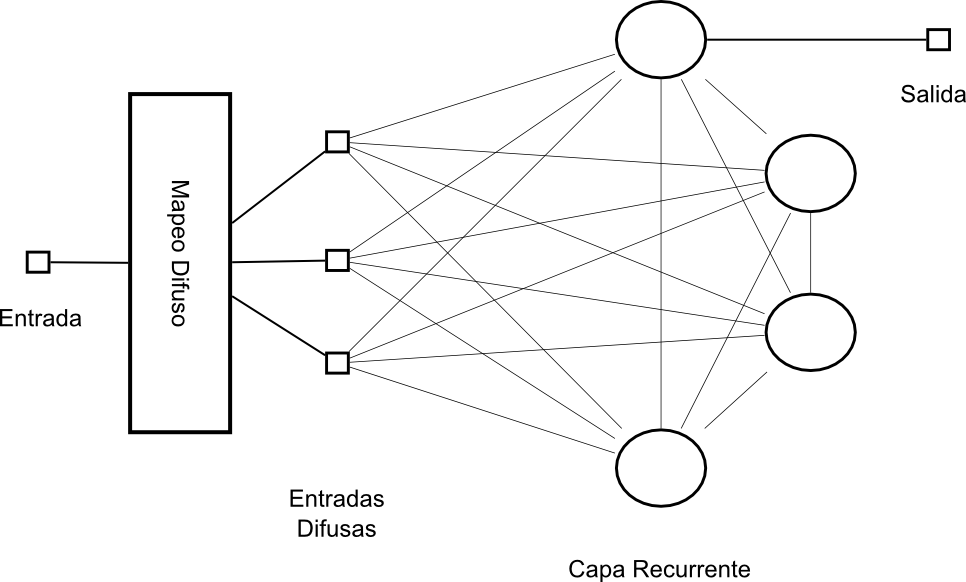
\includegraphics[width=7cm]{rnn.png}
  \caption{Neural net for stability control including fuzzy mapping}
  \label{rnn}
\end{figure}

\subsection*{Evolutionary Algorithm Structure for the RNN Controller}
It is expected, based on the approach of artificial life to
evolutionary robotics (Nolfi y Floreano), that the sequential and
cooperative evolution of elements with biological similarity leads to
an specialization in the process of stabilization and positioning
(despite the antagonistic individual goals of each controller because
of the interest of the positioning controller to maximize also the
global performance).

As said, the two steps are executed sequentially, taking the best
individual of the first step to collaborate with the individual
evolved in the second step.

Aiming to obtain a fixed length representation and limit the problem
dimensionality, it is used a model of order $Q$ totally connected. Any
network with an order equal or lesser and with total or partial
connections can be represented by the proposed model, by the addition
of activating/deactivating elements for neurons and
connections. Therefore, individual are codified as:

\begin{itemize}
\item A bit sequence representing a serialization of an activation
  matrix $A_a$ of dimension $Q$-by-$Q$ which activates/deactivates a
  recurrent connection.
\item A sequence of real numbers representing a serialization of
  matrices $W_a$ and $W_b$, of dimension $Q$-by-$Q$ and $Q$-by-$(m+1)$
  respectively.
\end{itemize}

The $C$ matrix is not evolved because it is chosen arbitrarily only
one output (the first neuron).

The evolution operations used in both steps are:
\begin{itemize}
\item Parametric mutation of inputs: Gaussian modification of real
  codified matrix weights, which varies connection weights of inputs.
\item Parametric mutation of recurrences: Gaussian modification of
  real codified matrix weights, which varies connection weights of
  recurrences.
\item Selection: Calculates population fitness, selects with elitism
  and culling (5\% of both) couples of parents for generating new
  offsprings, calculates the fitness function for both offsprings.
\end{itemize}

The fitness functions used are the same presented for the neural field
controller.

\section{Experimentation}
\subsection*{Experimentation Parameters}
The sampling time used was 0.04s (for neural networks and
visualization) and were performed 20s tests.

The differential equation system was solved by a numerical method, 4th
Order Runge-Kutta. The iteration step selected was $h=0.002s$ for each
test.

\subsection*{Results}
The first experiment tests the physical model using both controllers
without evolution, to see the natural dynamics of the system whit the
controller configured arbitrarily (in such a way that can be perceived
the action of the algorithm). Results are shown in the figure
\ref{inestabilidad}. As can be seen, it is an unstable system in the
origin. Red dots represent the pendulum position referenced to
universal coordinates, and blue dots represent the base (car)
position.


\begin{figure}[t]
  \centering
  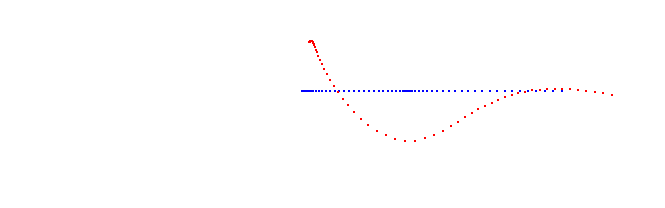
\includegraphics[width=7cm]{inestabilidadG.png}
  \\
  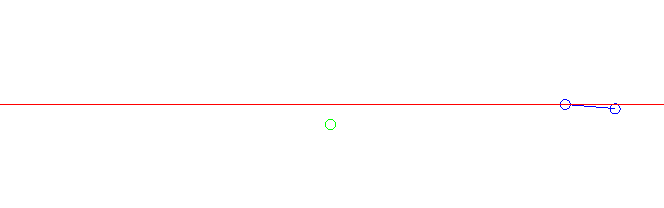
\includegraphics[width=7cm]{inestabilidadC.png}
  \caption{System dynamics with an untrained controller}
  \label{inestabilidad}
\end{figure}

After the first step of the algorithm, and once done the stability
controller evolution, it is shown the behavior withdrawing the
positioning controller in the figure \ref{estabilidad}. The evolution
was performed with a population of 50 individuals and 300 iterations.


\begin{figure}[t]
  \centering
  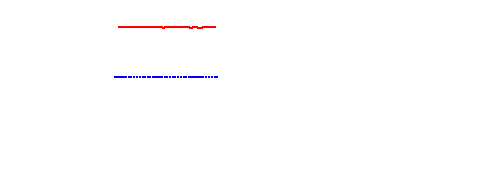
\includegraphics[width=7cm]{estabilidadG.png}
  \\
  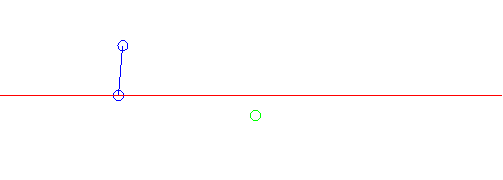
\includegraphics[width=7cm]{estabilidadC.png}
  \caption{System dynamics with a trained controller. Without
    reference tracking.}
  \label{estabilidad}
\end{figure}

Later, it was applied the second step of the algorithm. It was
connected the positioning controller and fixed the stability
controller (which is the best one of the previous step). It was
obtained the final performance shown in the figure \ref{final}.


\begin{figure}[t]
  \centering
  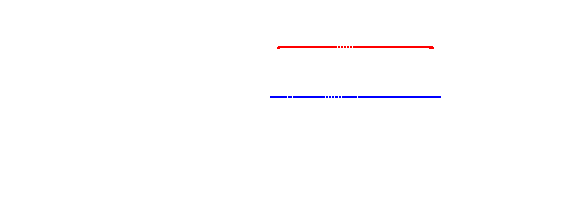
\includegraphics[width=7cm]{finalG.png}
  \\
  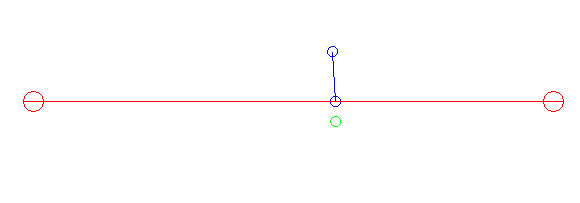
\includegraphics[width=7cm]{finalC.png}
  \caption{System dynamics with both controllers trained. Suitable
    behavior.}
  \label{final}
\end{figure}


\section{Conclusions}
% Finalmente, podemos concluir que el método presenta un balance
% entre una baja complejidad computacional y un rendimiento
% considerablemente bueno, siendo una alternativa a las técnicas de
% control que ubican mayormente la carga de diseño al experto
% humano. Así mismo, es notable la ratificación obtenida para el
% modelo en etapas de la evolución de la caminata bípeda
% simplificada, compuesta por una etapa de evolución de una red
% neuronal recurrente de estabilización, y otra etapa de evolución
% de una segunda red neuronal recurrente (que se diseña para
% colaborar con mejor red obtenida de la primera etapa) de
% posicionamiento.

\begin{thebibliography}{}
\bibitem[RN] {RN} Stuart Russell and Peter Norvig (2003)
  \textit{Artificial Intelligence: A Modern Approach}. Prentice-Hall,
  Englewood Cliffs, NJ.
\bibitem[Ha] {Ha} Simon Haykin (1994) \textit{Neural networks: a
    comprehensive foundation} Macmillan.
\bibitem[NF] {NF} Stefano Nolfi and Dario Floreano (2004)
  \textit{Evolutionary Robotics: The Biology, Intelligence, and
    Technology of Self-Organizing Machines} Bradford Book.
\end{thebibliography}

\end{document}
